\documentclass[12pt,a4paper]{article}

\usepackage[UTF8]{ctex}
\usepackage{amsmath,amscd,amsbsy,amssymb,latexsym,url,bm,amsthm}
\usepackage{amsfonts}
\usepackage{epsfig,graphicx,subfigure}
\usepackage{hyperref}
\usepackage{listings}
\usepackage[vlined,ruled,linesnumbered]{algorithm2e}
\usepackage{enumitem}
\usepackage{xcolor}
\usepackage{geometry}

%\uppercase\expandafter{\romannumeral1}:% 罗马数字。

\lstset{
language=Matlab,
keywordstyle= \color{blue!70},
commentstyle= \color{red!50!green!50!blue!50},
breaklines
}%设置listing插入语言

\setlength{\parindent}{0em}
\setlength{\parskip}{1em}

\geometry{bottom =3cm}
\newcommand{\textbi}[1]{%
\textbf{\textit{#1}}}

\newcommand{\ncolor}[1]{%
{\color[RGB]{139,117,0}{#1}}}
\newtheorem{theorem}{Theorem}[section]
\newenvironment{solution}{{\noindent \it \textbf{Solution:}}\\}

\title{MCM daily}
\author{Yunlong Cheng}

\begin{document}
\maketitle
\section{model learning}
\subsection{马尔萨斯-指数增长模型}
\begin{enumerate}
  \item 背景:今年人口$x_0$,年增长率$r$,预测$k$年后人口。
  \item 计算公式: $x_k = x_0(1+r)^k$.
  \item 推导:
  \begin{itemize}
    \item 基本假设: 人口相对增长率$r$是常数。
  \end{itemize}
  \begin{equation*}
    \begin{split}
      \frac{dx}{dt} &= rx \\
      x(0) &= x_0 \\
      x(t) &= x_0e^{rt} \\
      x(t) &= x_0(e^r)^t \approx x_0(1+r)^t
    \end{split}
  \end{equation*}
\end{enumerate}

\subsection{阻滞增长模型(Logistic模型)}
\begin{enumerate}
  \item 背景: 人口增长到一定程度后,增长率会下降。
  \item 假设:
  \begin{itemize}
    \item $r(x)=r-sx(r,s>0)$,$r$为与x有关的固有增长率。
    \item $x_m$为最大人口容量,则有$r(x_m) = 0$, $s = \frac{r}{x_m}$, $r(x)=r(1-\frac{x}{x_m})$。
  \end{itemize}
  \item 推导:
  \begin{equation*}
    \begin{split}
      \frac{dx}{dt}& = r(x)x = rx(1-\frac{x}{x_m})\\
      x(t)& = \frac{x_m}{1+(\frac{x_m}{x_0} - 1)e^{-rt}}
    \end{split}
  \end{equation*}
\end{enumerate}

\subsection{线性规划}
MATLAB中的线性规划有标准形式:
$$min\; \textbf{c}^T\textbf{x}\quad \textbf{Ax}\le b$$
其中$\textbf{c}$和$\textbf{x}$为$n$维列向量;$\textbf{b}$为$m$维列向量;$\textbf{A}$为$m\times n$矩阵。\\
基本函数形式为 linprog(c, A, b),返回值为向量$x$的值。

[x,fval] = linprog(c,A,b,Aeq,beq,Lb,Ub,X0,OPTIONS)

例题:
\begin{center}
  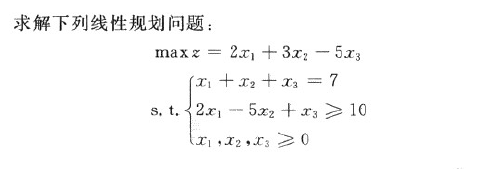
\includegraphics[width=\textwidth]{figures/LP_example}
\end{center}
解:\\
见\href{run:matlab/simple_lp.m}{matlab文件}.
\begin{table}[!htbp]
  \caption{c for this LP problem}
  \centering
  \begin{tabular}{|c|}
    c\\
    \hline
    2\\
    \hline
    3\\
    \hline
    -5
  \end{tabular}
\end{table}




\section{algorithm learning}
none

\section{MATLAB 基础使用方法}
\subsection{创建符号变量}
\begin{enumerate}
  \item 创建符号变量x和y:
  \begin{lstlisting}
    syms x y % syms can insert many variables.
    % Equals to the next two lines.
    x=sym('x')
    y=sym('y')
  \end{lstlisting}
  \item 将$a+b$转化为符号表达式:
  \begin{lstlisting}
    sys('a+b')
  \end{lstlisting}
\end{enumerate}
\subsection{数据读入与读出}
\begin{itemize}
  \item 与excel数据交互要安装 Spreadsheet Link,然后改动excel加载项。
\end{itemize}
\subsection{数据拟合方法}
\begin{enumerate}
  \item polyfit(X, Y, N): 多项式拟合。
  \item polyval(P, xi): 计算多项式的值。
  \item fittype: 自定义拟合函数. 示例:
  \begin{lstlisting}
  f=fittype('a * cos(k*t)*exp(w*t)','independent','t','coefficients',{'a','k','w'});
  \end{lstlisting}
  \item fit(x, y, f): 根据自定义拟合函数f拟合数据$x,y$.
\end{enumerate}
\end{document}
